%% ============================================================================
%% AD7031 Week 4 -- LECTURE NOTE
%%
%% Probability review, merged from two sources:
%%   - week 2 note, Sections 7-8 (this course's own prose, examples, figures)
%%   - G. Hanasusanto, "Optimization Under Uncertainty" (ORI397, UT Austin,
%%     Fall 2016), Section 1.2 -- events and conditioning, the scenario list,
%%     and expectation written once as an integral against P.
%%
%% Sample space is Omega here, not S: S counts scenarios from Section 3 on.
%% Same house style as OUU_week02_note.tex; self-contained -- no \input.
%% ============================================================================
\documentclass[10pt]{article}

\usepackage[a4paper, margin=1.9cm]{geometry}
\usepackage{amsmath, amssymb}
\usepackage[dvipsnames]{xcolor}
\usepackage{graphicx}
\usepackage{array}
\usepackage{tikz}
\usepackage[hidelinks]{hyperref}

\definecolor{ruleink}{RGB}{18, 68, 140}
\definecolor{demoink}{RGB}{140, 82, 20}
\definecolor{keyink}{RGB}{20, 90, 20}
\definecolor{watchink}{RGB}{86, 60, 140}
\definecolor{punchink}{RGB}{170, 30, 60}
\definecolor{lineA}{RGB}{44, 110, 176}
\definecolor{lineB}{RGB}{168, 96, 32}
\definecolor{lineC}{RGB}{78, 62, 140}

\setlength{\parindent}{0pt}
\pagestyle{empty}

% tighter spacing around centered displays
\AtBeginDocument{%
  \abovedisplayskip=7pt plus 2pt
  \belowdisplayskip=7pt plus 2pt
  \abovedisplayshortskip=4pt
  \belowdisplayshortskip=4pt}

% ---- one section -----------------------------------------------------------
\newcommand{\beat}[2]{%   number, title
  \par\bigskip\vspace{4pt}
  {\color{ruleink}\rule{\textwidth}{1pt}}\par\nobreak\vspace{4pt}
  {\large\bfseries #1.\; #2}\par\nobreak\vspace{6pt}}

% ---- board content ---------------------------------------------------------
\newenvironment{board}{%
  \par\vspace{4pt}
  \begingroup\leftskip=1.3em\relax\parskip=2pt\relax}{%
  \par\endgroup\vspace{4pt}}

% ---- highlights ------------------------------------------------------------
% ---- short rule used to draw a row vector inside a matrix ------------------
\newcommand{\rowline}{\rule[0.55ex]{1.15em}{0.4pt}}

% ---- hanging bullet (wrapped lines stay indented) --------------------------
\newcommand{\bul}{\hangindent=2.6em\hangafter=1\hspace{1.2em}\textbullet\ \ignorespaces}

\newcommand{\demo}[2]{\par{\color{demoink}\small\textbf{demo}\quad\texttt{#1} --- #2}\par}
\newcommand{\watch}[1]{\par{\color{watchink}\small\textbf{watch}\quad #1}\par}
\newcommand{\key}[1]{\par\vspace{1pt}{\color{keyink}\small\textbf{KEY}\quad\textbf{#1}}\par}
\newcommand{\takeaway}[1]{%
  \par\vspace{6pt}\noindent
  {\color{punchink}\rule{2pt}{10pt}}\;{\color{punchink}\small\textbf{takeaway}\quad\textbf{#1}}\par\vspace{2pt}}

\begin{document}

{\Large\bfseries Week 4 --- Probability Review, and the Markowitz Portfolio}\\[2pt]
{\small AD7031 Optimization Under Uncertainty \quad\textbullet\quad Instructor: Prof.\ H.\ Park \quad\textbullet\quad Sep 19, 2026}

%% ------------------------------------------------------------------ 1
\beat{1}{Random variables}
\begin{board}
back to week 2's Section 2 table: the OR column had \textbf{uncertain data} $\xi$. today, the vocabulary ---
textbook notation ($X$, $f$) first, this course's notation ($\tilde\xi$) at the end.
\vspace{10pt}

\textbf{Random variable}
\vspace{4pt}

\bul \textbf{random experiment:} its outcome is not known in advance
\vspace{3pt}

\bul \textbf{sample space} $\Omega$ = the set of all possible outcomes
\vspace{2pt}

\quad {\footnotesize\color{punchink}(week 2 wrote this $S$; from here it is $\Omega$, so that $S$ can count \emph{scenarios} below)}
\vspace{6pt}

\textbf{Def} (\emph{random variable}) \quad a function that assigns a real number to each outcome: \quad $X : \Omega \to \mathbb{R}$
\vspace{3pt}

\quad capital $X$ = the random variable, \qquad lowercase $x$ = a value it takes
\vspace{5pt}

\quad toss a coin twice: \ $\Omega = \{HH, HT, TH, TT\}$, \ each outcome has probability $\tfrac14$
\vspace{3pt}

\quad $X$ = number of heads: \quad $X(HH) = 2, \quad X(HT) = 1, \quad X(TH) = 1, \quad X(TT) = 0$
\vspace{6pt}

\begin{center}
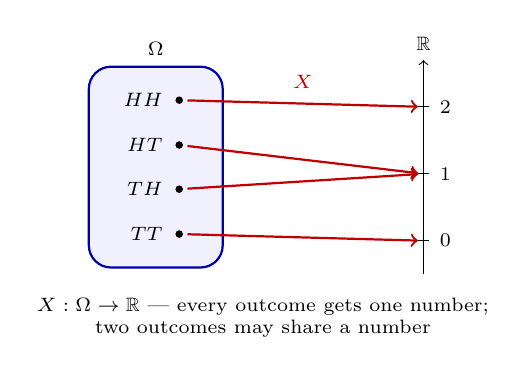
\begin{tikzpicture}[scale=0.85, font=\scriptsize]
  \draw[rounded corners=8pt, fill=blue!6, draw=blue!65!black, thick] (0,0) rectangle (2.0,3.0);
  \node[anchor=south] at (1.0,3.02) {$\Omega$};
  \foreach \y/\lab in {2.5/HH, 1.83/HT, 1.17/TH, 0.5/TT}
    { \fill (1.35,\y) circle (1.6pt); \node[anchor=east] at (1.25,\y) {$\lab$}; }
  \draw[->] (5.0,-0.1) -- (5.0,3.1) node[above] {$\mathbb{R}$};
  \foreach \v/\y in {0/0.4, 1/1.4, 2/2.4}
    { \draw (4.92,\y) -- (5.08,\y); \node[anchor=west] at (5.1,\y) {$\v$}; }
  \draw[->, red!75!black, thick, shorten >=2pt, shorten <=3pt] (1.35,2.5)  -- (5.0,2.4);
  \draw[->, red!75!black, thick, shorten >=2pt, shorten <=3pt] (1.35,1.83) -- (5.0,1.4);
  \draw[->, red!75!black, thick, shorten >=2pt, shorten <=3pt] (1.35,1.17) -- (5.0,1.4);
  \draw[->, red!75!black, thick, shorten >=2pt, shorten <=3pt] (1.35,0.5)  -- (5.0,0.4);
  \node[red!75!black] at (3.2,2.78) {$X$};
  \node[align=center] at (2.6,-0.75) {$X : \Omega \to \mathbb{R}$ --- every outcome gets one number;\\ two outcomes may share a number};
\end{tikzpicture}
\hspace{12mm}
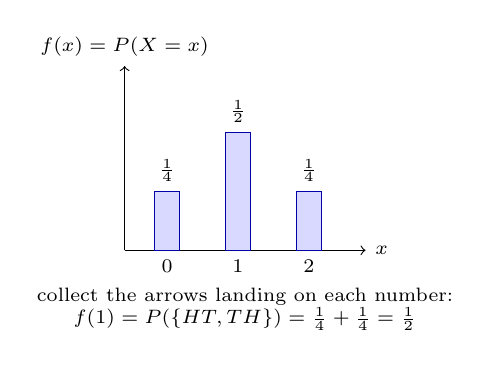
\begin{tikzpicture}[xscale=0.9, yscale=3.0, font=\scriptsize]
  \draw[->] (-0.6,0) -- (2.8,0) node[right] {$x$};
  \draw[->] (-0.6,0) -- (-0.6,0.78) node[above] {$f(x) = P(X = x)$};
  \draw[fill=blue!15, draw=blue!65!black] (-0.18,0) rectangle (0.18,0.25);
  \draw[fill=blue!15, draw=blue!65!black] (0.82,0) rectangle (1.18,0.5);
  \draw[fill=blue!15, draw=blue!65!black] (1.82,0) rectangle (2.18,0.25);
  \node[below] at (0,0) {$0$}; \node[below] at (1,0) {$1$}; \node[below] at (2,0) {$2$};
  \node[above, font=\tiny] at (0,0.25) {$\tfrac14$};
  \node[above, font=\tiny] at (1,0.5) {$\tfrac12$};
  \node[above, font=\tiny] at (2,0.25) {$\tfrac14$};
  \node[align=center] at (1.1,-0.25) {collect the arrows landing on each number:\\ $f(1) = P(\{HT, TH\}) = \tfrac14 + \tfrac14 = \tfrac12$};
\end{tikzpicture}
\end{center}
\vspace{6pt}

\bul \textbf{discrete} $X$: countably many values --- number of defective parts, number of arrivals, demand
\vspace{3pt}

\bul \textbf{continuous} $X$: values fill an interval --- length, time, temperature, a return
\vspace{14pt}
\end{board}
\beat{2}{Events, conditioning, independence}
\begin{board}
an \textbf{event} is a subset of the sample space, \ $A \subseteq \Omega$; \ $P(A)$ is the probability it occurs.
\vspace{6pt}

\bul \ $0 \le P(A) \le 1$, \qquad $P(\Omega) = 1$
\vspace{3pt}

\bul \ $P(A \cup B) = P(A) + P(B) - P(A \cap B)$ \qquad --- subtract the overlap, or it is counted twice
\vspace{10pt}

\textbf{Def} (\emph{conditional probability}) \quad
$P(A \mid B) = \dfrac{P(A \cap B)}{P(B)}$, \qquad defined when $P(B) > 0$
\vspace{3pt}

\quad --- $B$ becomes the new sample space; divide by $P(B)$ so the weights add to $1$ again
\vspace{10pt}

\textbf{Def} (\emph{independent events}) \quad $A$ and $B$ are independent if \quad $P(A \cap B) = P(A)\,P(B)$
\vspace{3pt}

\quad then \ $P(A \mid B) = \dfrac{P(A)\,P(B)}{P(B)} = P(A)$ \quad --- learning $B$ tells you nothing about $A$
\vspace{10pt}

\textbf{Thm} (\emph{law of total probability}) \quad let $A_1, \dots, A_I$ \textbf{partition} $\Omega$:
\ $A_i \cap A_j = \emptyset$ for $i \ne j$, \ and \ $\bigcup_{i} A_i = \Omega$. \ then for any event $B$,
\[
P(B) \;=\; P(B \cap A_1) + \cdots + P(B \cap A_I)
     \;=\; P(B \mid A_1)\,P(A_1) + \cdots + P(B \mid A_I)\,P(A_I)
\]

\quad --- split the world into cases, answer each case, weight by how likely the case is
\vspace{10pt}

\quad two coins again. \ $A_1$ = first toss is $H$, \ $A_2$ = first toss is $T$ --- a partition, each of probability $\tfrac12$
\vspace{4pt}

\quad take $B = \{X \ge 1\}$: \qquad $P(B \mid A_1) = 1$ \ (a head already landed), \qquad
      $P(B \mid A_2) = \tfrac12$ \ (needs the second)
\vspace{4pt}

\quad $P(B) = 1 \cdot \tfrac12 \;+\; \tfrac12 \cdot \tfrac12 \;=\; \tfrac34$ \qquad
      --- the same $\tfrac34$ the PMF gives in Section 3
\end{board}
\takeaway{conditioning is how a \emph{two-stage} decision gets written down: act, watch which $A_i$ occurred, act again. weeks 10--12 run on this.}

%% ------------------------------------------------------------------ 3
\beat{3}{Discrete random variables}
\begin{board}
\textbf{Def} (\emph{probability mass function, PMF}) \quad
$f(x) = P(X = x)$, \qquad $f : \mathbb{R} \to [0,1]$
\vspace{3pt}

\quad (1) \ $f(x) \ge 0$ \qquad (2) \ $\sum_x f(x) = 1$ \qquad\qquad $P(X \in A) = \sum_{x \in A} f(x)$
\vspace{3pt}

\quad two coins: \ $f(0) = \tfrac14$, \ $f(1) = \tfrac12$, \ $f(2) = \tfrac14$, \qquad
$P(X \ge 1) = f(1) + f(2) = \tfrac34$

\vspace{10pt}

\textbf{The same object, this course's way} \quad a discrete random variable is a \textbf{list of scenarios} with weights:
\vspace{4pt}

\quad $\tilde\xi$ takes the values $\xi_1, \dots, \xi_S$ \ with \ $p_s = \mathbb{P}(\tilde\xi = \xi_s)$, \qquad
$p_s \ge 0$, \qquad $\sum_{s \in [S]} p_s = 1$
\vspace{3pt}

\quad here $[S] = \{1, \dots, S\}$ \ and \ $s$ indexes \emph{scenarios} --- $S$ of them, listed out
\vspace{4pt}

\quad two coins: \ three scenarios \ $\xi_1 = 0$, \ $\xi_2 = 1$, \ $\xi_3 = 2$ \ with \ $p = \big(\tfrac14, \tfrac12, \tfrac14\big)$
\vspace{4pt}

\quad {\color{punchink}same content as the PMF, different packaging.} \ a PMF is a function; a scenario list is a
      \emph{table} --- and a solver can only be handed a table. every model from week 10 on is written this way.

\vspace{8pt}

\textbf{Def} (\emph{mean, variance})
\vspace{3pt}

\quad mean: \quad $\mu = \mathbb{E}[X] = \sum_x x\, f(x)$
\vspace{3pt}

\quad variance: \quad $\sigma^2 = \mathrm{Var}(X) = \sum_x (x - \mu)^2 f(x) = \mathbb{E}[X^2] - \mu^2$,
\qquad standard deviation \ $\sigma = \sqrt{\mathrm{Var}(X)}$
\vspace{3pt}

\quad function of $X$: \quad $\mathbb{E}[h(X)] = \sum_x h(x)\, f(x)$
\qquad {\color{punchink}\small $\leftarrow$ law of the unconscious statistician}
\vspace{3pt}

\quad $\mathbb{E}[aX + b] = a\,\mathbb{E}[X] + b$, \qquad $\mathrm{Var}(aX + b) = a^2\,\mathrm{Var}(X)$
\vspace{10pt}

\textbf{Example 1} \quad demand $X$ for a spare part next month:
\vspace{5pt}

\begin{center}
\begin{tabular}{@{}l|ccc@{}}
 $x$     & 4    & 8   & 12   \\ \hline
 $f(x)$  & 0.25 & 0.5 & 0.25 \\
\end{tabular}
\qquad\qquad
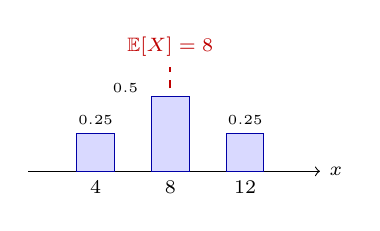
\begin{tikzpicture}[scale=0.95, font=\scriptsize, baseline=-6pt]
  \draw[dashed, red!75!black, thick] (1.6,0) -- (1.6,1.4) node[above] {$\mathbb{E}[X] = 8$};
  \draw[->] (-0.3,0) -- (3.6,0) node[right] {$x$};
  \draw[fill=blue!15, draw=blue!65!black] (0.35,0) rectangle (0.85,0.5);
  \draw[fill=blue!15, draw=blue!65!black] (1.35,0) rectangle (1.85,1.0);
  \draw[fill=blue!15, draw=blue!65!black] (2.35,0) rectangle (2.85,0.5);
  \node[below] at (0.6,0) {4}; \node[below] at (1.6,0) {8}; \node[below] at (2.6,0) {12};
  \node[font=\tiny] at (0.6,0.68) {$0.25$}; \node[font=\tiny, anchor=east] at (1.30,1.12) {$0.5$}; \node[font=\tiny] at (2.6,0.68) {$0.25$};
\end{tikzpicture}
\end{center}
\vspace{5pt}

\quad $\mathbb{E}[X] = 0.25 \cdot 4 + 0.5 \cdot 8 + 0.25 \cdot 12 = 8$
\vspace{3pt}

\quad $\mathrm{Var}(X) = 0.25 \cdot (4 - 8)^2 + 0.5 \cdot (8 - 8)^2 + 0.25 \cdot (12 - 8)^2 = 8$,
\qquad $\sigma = 2\sqrt{2} \approx 2.83$
\vspace{14pt}
\end{board}
%% ------------------------------------------------------------------ 4
\beat{4}{Continuous random variables}
\begin{board}
\textbf{Def} (\emph{probability density function, PDF}) \quad $f : \mathbb{R} \to \mathbb{R}_+$ with
\vspace{3pt}

\quad (1) \ $f(x) \ge 0$ \qquad (2) \ $\int_{-\infty}^{\infty} f(x)\, dx = 1$ \qquad
(3) \ $P(a \le X \le b) = \int_a^b f(x)\, dx$ \ = area under $f$ from $a$ to $b$
\vspace{3pt}

\quad {\color{punchink}$f(x)$ is \emph{not} a probability:} \ $P(X = x) = 0$ for every single $x$, \ and $f(x) > 1$ is allowed
\vspace{8pt}

\textbf{Def} (\emph{mean, variance}) \quad same as discrete --- the sums become integrals:
\vspace{3pt}

\quad $\mu = \mathbb{E}[X] = \int x\, f(x)\, dx$, \qquad
$\sigma^2 = \mathrm{Var}(X) = \int (x - \mu)^2 f(x)\, dx = \mathbb{E}[X^2] - \mu^2$, \qquad
$\mathbb{E}[h(X)] = \int h(x)\, f(x)\, dx$
\vspace{10pt}

\textbf{Example 2} \quad $X \sim \mathrm{Uniform}[a,b]$ \ ---
$f(x) = \dfrac{1}{b-a}$ \ on \ $[a,b]$, \ $0$ outside
\vspace{4pt}

\begin{center}
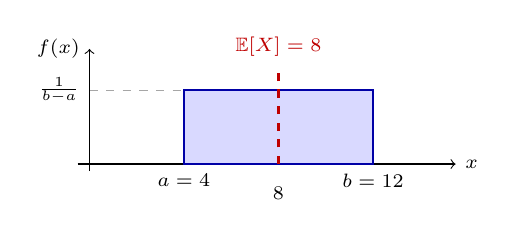
\begin{tikzpicture}[xscale=0.30, yscale=7.5, font=\scriptsize]
  \draw[dashed, gray!70] (0,0.125) -- (4,0.125);
  \draw[->] (-0.5,0) -- (15.5,0) node[right] {$x$};
  \draw[->] (0,-0.012) -- (0,0.195) node[left] {$f(x)$};
  \draw[fill=blue!15, draw=blue!65!black, thick] (4,0) rectangle (12,0.125);
  \node[below] at (4,0) {$a = 4$};
  \node[below] at (12,0) {$b = 12$};
  \node[left] at (0,0.125) {$\tfrac{1}{b-a}$};
  \draw[dashed, red!75!black, thick] (8,0) -- (8,0.165) node[above] {$\mathbb{E}[X] = 8$};
  \node[below] at (8,-0.022) {$8$};
\end{tikzpicture}
\end{center}
\vspace{4pt}

\quad mean:
\[
\mathbb{E}[X] \;=\; \int_a^b x \, \frac{1}{b-a} \, dx
 \;=\; \frac{1}{b-a}\left[\frac{x^2}{2}\right]_a^b
 \;=\; \frac{b^2 - a^2}{2(b-a)} \;=\; \frac{a+b}{2}
\]

\quad second moment --- $h(x) = x^2$:
\[
\mathbb{E}[X^2] \;=\; \int_a^b x^2 \, \frac{1}{b-a} \, dx
 \;=\; \frac{1}{b-a}\left[\frac{x^3}{3}\right]_a^b
 \;=\; \frac{b^3 - a^3}{3(b-a)} \;=\; \frac{a^2 + ab + b^2}{3}
\]

\quad variance --- subtract, no new integral:
\[
\mathrm{Var}(X) \;=\; \mathbb{E}[X^2] - \mathbb{E}[X]^2
 \;=\; \frac{a^2 + ab + b^2}{3} - \frac{(a+b)^2}{4}
 \;=\; \frac{(b-a)^2}{12}
\]

\quad with $a = 4$, $b = 12$: \qquad
$\mathbb{E}[X] = 8$, \qquad
$\mathrm{Var}(X) = \dfrac{64}{12} = \dfrac{16}{3}$, \qquad
$\sigma = \dfrac{4}{\sqrt{3}} \approx 2.31$
\vspace{12pt}

\textbf{Normal distribution} \quad $X \sim \mathcal{N}(\mu, \sigma^2)$:
\qquad $f(x) = \dfrac{1}{\sigma\sqrt{2\pi}}\, \exp\!\Big(\!-\dfrac{(x-\mu)^2}{2\sigma^2}\Big)$, \ $x \in \mathbb{R}$
\vspace{4pt}

\quad $\mathbb{E}[X] = \mu$, \qquad $\mathrm{Var}(X) = \sigma^2$
\vspace{3pt}

\quad $P(\mu - \sigma \le X \le \mu + \sigma) \approx 0.68$, \qquad
$P(\mu - 2\sigma \le X \le \mu + 2\sigma) \approx 0.95$
\vspace{4pt}

\begin{center}
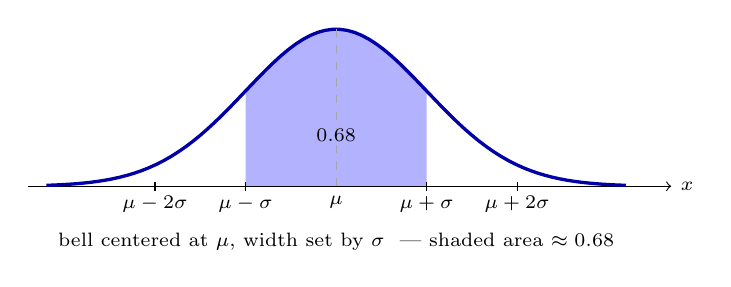
\begin{tikzpicture}[xscale=1.15, yscale=5.0, font=\scriptsize]
  \fill[blue!30, domain=-1:1, samples=40] (-1,0) -- plot (\x, {0.3989*exp(-\x*\x/2)}) -- (1,0) -- cycle;
  \draw[->] (-3.4,0) -- (3.7,0) node[right] {$x$};
  \draw[very thick, blue!65!black, domain=-3.2:3.2, samples=80] plot (\x, {0.3989*exp(-\x*\x/2)});
  \draw[dashed, gray!70] (0,0) -- (0,0.3989);
  \foreach \t in {-2,-1,1,2} \draw (\t,0.012) -- (\t,-0.012);
  \node[below] at (0,0) {$\mu$};
  \node[below] at (-1,0) {$\mu - \sigma$}; \node[below] at (1,0) {$\mu + \sigma$};
  \node[below] at (-2,0) {$\mu - 2\sigma$}; \node[below] at (2,0) {$\mu + 2\sigma$};
  \node at (0,0.13) {$0.68$};
  \node at (0,-0.14) {bell centered at $\mu$, width set by $\sigma$ \ --- shaded area $\approx 0.68$};
\end{tikzpicture}
\end{center}
\vspace{14pt}
\end{board}
\beat{5}{Expectation, in one formula}
\begin{board}
Sections 3 and 4 defined the mean twice --- once a sum, once an integral. one definition covers both.
\vspace{10pt}

\textbf{Def} (\emph{expectation}) \quad for $\tilde\xi \sim \mathbb{P}$,
\[
\mathbb{E}_{\mathbb{P}}\big[\tilde\xi\big] \;=\; \int_{\Omega} \xi \;\, \mathbb{P}(d\xi)
\]

\quad read $\mathbb{P}(d\xi)$ as \emph{the probability sitting on a small piece} $d\xi$ --- the weight, whichever form it takes:
\vspace{6pt}

\begin{center}
\renewcommand{\arraystretch}{1.3}
\begin{tabular}{@{}l|l|l@{}}
                & the weight $\mathbb{P}(d\xi)$ is        & and $\mathbb{E}_{\mathbb{P}}[\tilde\xi]$ reads \\ \hline
discrete        & $p_s$, \ one per scenario $\xi_s$       & $\sum_{s \in [S]} p_s\, \xi_s$ \\
continuous      & $p(\xi)\, d\xi$                         & $\int_{\Xi} \xi\, p(\xi)\, d\xi$ \\
\end{tabular}
\end{center}
\vspace{10pt}

\textbf{Def} (\emph{expectation of a function}) \quad for $f : \mathbb{R}^k \to \mathbb{R}$ and a random vector $\tilde\xi$,
\[
\mathbb{E}_{\mathbb{P}}\big[f(\tilde\xi)\big] \;=\; \int_{\Omega} f(\xi) \;\, \mathbb{P}(d\xi)
\qquad\text{---}\qquad
\sum_{s \in [S]} p_s\, f(\xi_s)
\quad\text{or}\quad
\int_{\Xi} f(\xi)\, p(\xi)\, d\xi
\]

\quad {\color{punchink}this is the one the course actually needs:} \ $f$ will be a \textbf{cost}, and $\mathbb{E}[f(x, \tilde\xi)]$ the objective.
\vspace{10pt}

\quad variance is an expectation too, so it inherits the same two readings:
\vspace{4pt}

\quad $\mathrm{Var}(\tilde\xi) = \mathbb{E}\big[(\tilde\xi - \mathbb{E}[\tilde\xi])^2\big]$, \qquad
      $\sigma(\tilde\xi) = \sqrt{\mathrm{Var}(\tilde\xi)}$, \qquad
      $\mathrm{Cov}(\tilde\xi_1, \tilde\xi_2) = \mathbb{E}\big[(\tilde\xi_1 - \mathbb{E}[\tilde\xi_1])(\tilde\xi_2 - \mathbb{E}[\tilde\xi_2])\big]$
\end{board}
\takeaway{one definition, two computations. write $\mathbb{E}$ once and stop asking whether the data is discrete or continuous.}

%% ------------------------------------------------------------------ 6
\beat{6}{Two random variables}
\begin{board}
\textbf{Def} (\emph{joint PMF}) \quad
$f_{XY}(x, y) = P(X = x, \ Y = y)$, \qquad $f_{XY} \ge 0$, \qquad $\sum_x \sum_y f_{XY}(x, y) = 1$
\vspace{6pt}

\textbf{Def} (\emph{marginal PMF}) \quad
$f_X(x) = \sum_y f_{XY}(x, y)$, \qquad $f_Y(y) = \sum_x f_{XY}(x, y)$
\vspace{2pt}

\quad --- row sums and column sums, written in the \emph{margins} of the table
\vspace{10pt}

\textbf{Example 3} \quad two assets, returns tomorrow: \ $X$, $Y$ each either down ($-0.10$) or up ($+0.20$)
\vspace{6pt}

\begin{center}
\begin{tabular}{@{}c|cc|c@{}}
 $f_{XY}(x, y)$        & $y = -0.10$ & $y = 0.20$ & $f_X(x)$ \\ \hline
 $x = -0.10$           & $0.3$ & $0.2$ & $0.5$ \\
 $x = \phantom{-}0.20$ & $0.2$ & $0.3$ & $0.5$ \\ \hline
 $f_Y(y)$              & $0.5$ & $0.5$ & $1$ \\
\end{tabular}
\end{center}
\vspace{4pt}

\quad each asset alone: down or up w.p.\ $\tfrac12$. \quad together: same direction w.p.\ $0.3 + 0.3 = 0.6$
\vspace{10pt}

\textbf{Def} (\emph{joint PDF}) \quad
$f_{XY} : \mathbb{R}^2 \to \mathbb{R}_+$, \qquad $\iint f_{XY}(x, y)\, dx\, dy = 1$, \qquad
$P\big((X, Y) \in R\big) = \iint_R f_{XY}(x, y)\, dx\, dy$
\vspace{2pt}

\quad --- the \textbf{volume} under $f_{XY}$ above the region $R$
\vspace{3pt}

\quad marginal PDF: \ $f_X(x) = \int f_{XY}(x, y)\, dy$ \quad --- the sum becomes an integral
\vspace{10pt}

\textbf{Example 4} \quad $(X, Y)$ uniform on the unit square: \quad $f_{XY}(x, y) = 1$ \ on $[0,1]^2$, \ $0$ outside
\vspace{4pt}

\begin{center}
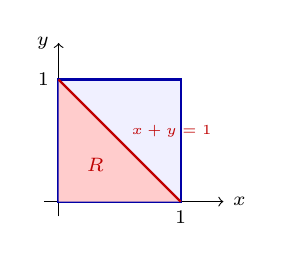
\begin{tikzpicture}[scale=1.55, font=\scriptsize, baseline=(b)]
  \coordinate (b) at (0,0.5);
  \draw[->] (-0.12,0) -- (1.35,0) node[right] {$x$};
  \draw[->] (0,-0.12) -- (0,1.3) node[left] {$y$};
  \draw[fill=blue!6, draw=blue!65!black, thick] (0,0) rectangle (1,1);
  \fill[red!20] (0,0) -- (1,0) -- (0,1) -- cycle;
  \draw[red!75!black, thick] (1,0) -- (0,1);
  \node[red!75!black] at (0.3,0.3) {$R$};
  \node[below] at (1,0) {$1$}; \node[left] at (0,1) {$1$};
  \node[anchor=west, font=\tiny, red!75!black] at (0.52,0.58) {$x + y = 1$};
\end{tikzpicture}
\qquad\quad
\begin{minipage}{0.62\textwidth}
$P(X + Y \le 1) = \iint_R 1 \; dx\, dy$ = area of the triangle $R$ $= \tfrac12$
\vspace{6pt}

marginal: \ $f_X(x) = \int_0^1 1 \; dy = 1$ on $[0,1]$ --- $X$ alone is Uniform$[0,1]$
\end{minipage}
\end{center}
\vspace{10pt}

\textbf{Def} (\emph{independence}) \quad $X$, $Y$ are independent if \quad
$f_{XY}(x, y) = f_X(x)\, f_Y(y) \quad \forall\, x, y$ \qquad (PMF or PDF)
\vspace{3pt}

\quad Example 3: \ $f_{XY}(-0.10, -0.10) = 0.3 \ne 0.5 \cdot 0.5$ \ --- \textbf{not} independent
\vspace{2pt}

\quad Example 4: \ $f_{XY}(x, y) = 1 = 1 \cdot 1$ \ --- independent
\vspace{10pt}
\end{board}
%% ------------------------------------------------------------------ 7
\beat{7}{Covariance and correlation}
\begin{board}
\textbf{Def} (\emph{covariance, correlation})
\vspace{3pt}

\quad $\mathrm{Cov}(X, Y) = \mathbb{E}\big[(X - \mu_X)(Y - \mu_Y)\big] = \mathbb{E}[XY] - \mu_X \mu_Y$,
\qquad $\mathrm{Cov}(X, X) = \mathrm{Var}(X)$
\vspace{3pt}

\quad $\rho_{XY} = \dfrac{\mathrm{Cov}(X, Y)}{\sigma_X\, \sigma_Y}$, \qquad $-1 \le \rho_{XY} \le 1$
\vspace{3pt}

\quad $\rho > 0$: move together, \quad $\rho < 0$: move opposite, \quad independent $\Rightarrow$ $\rho = 0$
\vspace{4pt}

\begin{center}
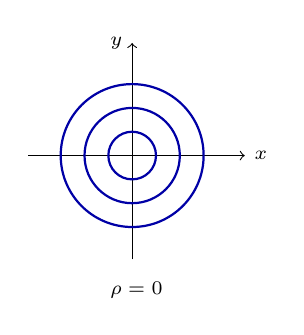
\begin{tikzpicture}[scale=0.55, font=\scriptsize]
  \draw[->] (-2.4,0) -- (2.6,0) node[right] {$x$};
  \draw[->] (0,-2.4) -- (0,2.6) node[left] {$y$};
  \foreach \c in {0.55,1.1,1.65}
    \draw[blue!65!black, thick] (0,0) circle (\c);
  \node at (0.1,-3.1) {$\rho = 0$};
\end{tikzpicture}
\hspace{9mm}
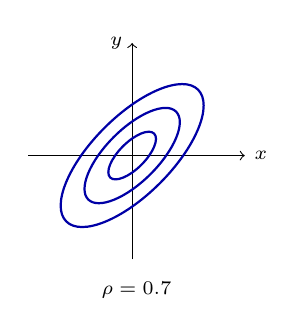
\begin{tikzpicture}[scale=0.55, font=\scriptsize]
  \draw[->] (-2.4,0) -- (2.6,0) node[right] {$x$};
  \draw[->] (0,-2.4) -- (0,2.6) node[left] {$y$};
  \foreach \c in {0.55,1.1,1.65}
    \draw[blue!65!black, thick, rotate=45] (0,0) ellipse ({1.304*\c} and {0.548*\c});
  \node at (0.1,-3.1) {$\rho = 0.7$};
\end{tikzpicture}
\hspace{9mm}
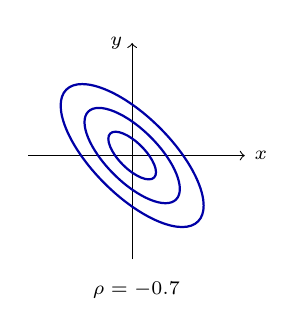
\begin{tikzpicture}[scale=0.55, font=\scriptsize]
  \draw[->] (-2.4,0) -- (2.6,0) node[right] {$x$};
  \draw[->] (0,-2.4) -- (0,2.6) node[left] {$y$};
  \foreach \c in {0.55,1.1,1.65}
    \draw[blue!65!black, thick, rotate=-45] (0,0) ellipse ({1.304*\c} and {0.548*\c});
  \node at (0.1,-3.1) {$\rho = -0.7$};
\end{tikzpicture}\\[2pt]
{\scriptsize contours of the joint PDF of two normal random variables, \ $\mu_X = \mu_Y = 0$, \ $\sigma_X = \sigma_Y = 1$}
\end{center}
\vspace{8pt}

\textbf{Example 3, continued} \quad (use the margins for $\mu$ and $\sigma$, all four cells for the covariance)
\vspace{4pt}

\quad $\mu_X = 0.5 \cdot (-0.10) + 0.5 \cdot 0.20 = 0.05$, \qquad $\mu_Y = 0.05$
\vspace{3pt}

\quad $\mathrm{Var}(X) = 0.5 \cdot (-0.15)^2 + 0.5 \cdot (0.15)^2 = 0.0225$, \qquad $\sigma_X = \sigma_Y = 0.15$
\[
\begin{aligned}
\mathrm{Cov}(X, Y)
 &= 0.3\,(-0.15)(-0.15) + 0.2\,(-0.15)(0.15) + 0.2\,(0.15)(-0.15) + 0.3\,(0.15)(0.15) \\
 &= (0.3 - 0.2 - 0.2 + 0.3) \cdot 0.0225 \;=\; 0.0045
\end{aligned}
\]

\quad $\rho_{XY} = \dfrac{0.0045}{0.15 \cdot 0.15} = 0.2$ \quad --- the two assets tend to move together
\vspace{14pt}
\end{board}
%% ------------------------------------------------------------------ 8
\beat{8}{Linear combinations}
\begin{board}
\quad $\mathbb{E}[aX + bY] = a\,\mu_X + b\,\mu_Y$ \qquad --- always, no independence needed
\vspace{3pt}

\quad $\mathrm{Var}(aX + bY) = a^2\,\mathrm{Var}(X) + b^2\,\mathrm{Var}(Y) + 2ab\,\mathrm{Cov}(X, Y)$
\vspace{8pt}

\quad $n$ random variables $X = (X_1, \dots, X_n)$:
\vspace{3pt}

\qquad mean vector \ $\mu = \big(\mathbb{E}[X_1], \dots, \mathbb{E}[X_n]\big)^{\top} \in \mathbb{R}^n$
\vspace{3pt}

\qquad covariance matrix \ $\Sigma \in \mathbb{R}^{n \times n}$, \ $\Sigma_{ij} = \mathrm{Cov}(X_i, X_j)$;
\ diagonal $\Sigma_{ii} = \mathrm{Var}(X_i)$; \ symmetric; \ always $\Sigma \succeq 0$
\vspace{4pt}

\quad for fixed $c \in \mathbb{R}^n$: \qquad
$\mathbb{E}[c^{\top}X] = c^{\top}\mu$, \qquad $\mathrm{Var}(c^{\top}X) = c^{\top}\Sigma c$
\vspace{4pt}

\quad $n = 2$, \ $c = (a, b)$: \quad
$c^{\top}\Sigma c
 = \begin{pmatrix} a & b \end{pmatrix}
   \begin{pmatrix} \mathrm{Var}(X) & \mathrm{Cov}(X,Y) \\ \mathrm{Cov}(X,Y) & \mathrm{Var}(Y) \end{pmatrix}
   \begin{pmatrix} a \\ b \end{pmatrix}$
\ --- $\mathrm{Var}(aX + bY)$ again
\vspace{4pt}

\quad Example 3: \quad
$\mu = \begin{pmatrix} 0.05 \\ 0.05 \end{pmatrix}$, \qquad
$\Sigma = \begin{pmatrix} 0.0225 & 0.0045 \\ 0.0045 & 0.0225 \end{pmatrix}$
\vspace{14pt}
\end{board}
%% ------------------------------------------------------------------ 9
\beat{9}{This course's notation, and the bridge}
\begin{board}
the decision is already $x$, so the uncertain data gets its own letter:
\vspace{5pt}

\begin{center}
\renewcommand{\arraystretch}{1.25}
\begin{tabular}{@{}l|l|l@{}}
                        & textbook                      & this course \\ \hline
random variable         & $X$                           & $\tilde\xi$, \ with distribution $\mathbb{P}$: \ $\tilde\xi \sim \mathbb{P}$ \\
a value of it           & $x$                           & $\xi$ \ (a \emph{realization}) \\
probability             & $P(\cdot)$                    & $\mathbb{P}(\cdot)$ \\
set of possible values  & range of $X$                  & support $\Xi$ \ (smallest closed set with $\mathbb{P}(\tilde\xi \in \Xi) = 1$) \\
discrete                & values $x$, PMF $f(x)$        & scenarios $\xi_1, \dots, \xi_S$ with probabilities $p_1, \dots, p_S$ \\
continuous              & PDF $f(x)$                    & density $p(\xi)$ \\
mean, discrete          & $\sum_x x\, f(x)$             & $\mathbb{E}[\tilde\xi] = \sum_{s \in [S]} p_s\, \xi_s$ \\
mean, continuous        & $\int x\, f(x)\, dx$          & $\mathbb{E}[\tilde\xi] = \int_{\Xi} \xi\, p(\xi)\, d\xi$ \\
function of it          & $\mathbb{E}[h(X)]$            & $\mathbb{E}[f(\tilde\xi)]$ \ ($f$ = any function, e.g.\ a cost --- not a PDF) \\
random vector           & $X \in \mathbb{R}^k$, \ $\mu$, $\Sigma$ & $\tilde\xi \in \mathbb{R}^k$, \ $\mu$, $\Sigma$ \\
\end{tabular}
\end{center}
\vspace{12pt}

\textbf{The bridge to optimization} \quad data random $\Rightarrow$ cost random:
$f(x, \tilde\xi)$ is a random variable, \ $\mathbb{E}[f(x,\tilde\xi)]$ is a number.
\[
\min_x \;\; \mathbb{E}\big[f(x, \tilde\xi)\big]
\]
\end{board}
\takeaway{every paradigm in this course differs in one place only: \emph{how} it collapses the randomness to a number.}
%% ------------------------------------------------------------------ 10
\beat{10}{Running example: the Markowitz portfolio}
\begin{board}
\begin{board}
a budget of $1$, \ $n$ assets. \quad decide the split today; the returns are revealed tomorrow.
\vspace{6pt}

\bul \textbf{decision:} \ $x \in \mathbb{R}^n$, \ $x_j$ = share of the budget in asset $j$
\vspace{3pt}

\bul \textbf{uncertain data:} \ $\tilde\xi = (\tilde\xi_1, \dots, \tilde\xi_n) \in \mathbb{R}^n$, \
      $\tilde\xi_j$ = return of asset $j$ \ --- a random vector with mean $\mu$, covariance matrix $\Sigma$
\vspace{3pt}

\bul \textbf{feasible set:} \ $X = \{\, x \in \mathbb{R}^n \;:\; \mathbf{1}^{\top}x = 1, \ x \ge 0 \,\}$
      \qquad ($\mathbf{1}$ = all-ones vector, \ $\mathbf{1}^{\top}x = x_1 + \cdots + x_n$)
\vspace{10pt}

\textbf{Portfolio return} \quad
$\tilde\xi^{\top}x = x_1\tilde\xi_1 + \cdots + x_n\tilde\xi_n$ \quad --- a random variable
\vspace{3pt}

\quad as a function: \ fix $x$, \quad $f(\xi) = \xi^{\top}x$, \quad $f : \mathbb{R}^n \to \mathbb{R}$
\quad --- Section 0's inner product, fed a random input
\vspace{3pt}

\quad loss: \ $f(x, \tilde\xi) = -\tilde\xi^{\top}x$ \qquad (a gain is a negative loss)
\vspace{6pt}

\quad Section 7's linear combinations with $c = x$: \qquad
$\mathbb{E}[\tilde\xi^{\top}x] = \mu^{\top}x$, \qquad $\mathrm{Var}(\tilde\xi^{\top}x) = x^{\top}\Sigma x$
\vspace{10pt}

\textbf{Check on Example 3} \quad $(\tilde\xi_1, \tilde\xi_2)$ = Example 3's $(X, Y)$, \ half in each: \ $x = (\tfrac12, \tfrac12)$
\vspace{4pt}

\begin{center}
\begin{tabular}{@{}cc|c|c@{}}
 $\xi_1$ & $\xi_2$ & $\tfrac12\xi_1 + \tfrac12\xi_2$ & probability \\ \hline
 $-0.10$ & $-0.10$ & $-0.10$ & $0.3$ \\
 $-0.10$ & $\phantom{-}0.20$ & $\phantom{-}0.05$ & $0.2$ \\
 $\phantom{-}0.20$ & $-0.10$ & $\phantom{-}0.05$ & $0.2$ \\
 $\phantom{-}0.20$ & $\phantom{-}0.20$ & $\phantom{-}0.20$ & $0.3$ \\
\end{tabular}
\qquad\quad $\Rightarrow$ \quad PMF of $\tilde\xi^{\top}x$: \quad
\begin{tabular}{@{}l|ccc@{}}
 value       & $-0.10$ & $0.05$ & $0.20$ \\ \hline
 probability & $0.3$   & $0.4$  & $0.3$  \\
\end{tabular}
\end{center}
\vspace{4pt}

\[
\begin{aligned}
\text{from the PMF:}\quad
 & \mathbb{E}[\tilde\xi^{\top}x] = 0.3\,(-0.10) + 0.4\,(0.05) + 0.3\,(0.20) = 0.05 \\
 & \mathrm{Var}(\tilde\xi^{\top}x) = 0.3\,(-0.15)^2 + 0.4\,(0)^2 + 0.3\,(0.15)^2 = 0.0135 \\[5pt]
\text{from $\mu$ and $\Sigma$:}\quad
 & \mu^{\top}x = \tfrac12\,(0.05) + \tfrac12\,(0.05) = 0.05 \ \checkmark \\
 & x^{\top}\Sigma x = \tfrac14\,(0.0225) + \tfrac14\,(0.0225) + 2 \cdot \tfrac14\,(0.0045) = 0.0135 \ \checkmark
\end{aligned}
\]
\vspace{2pt}

\begin{center}
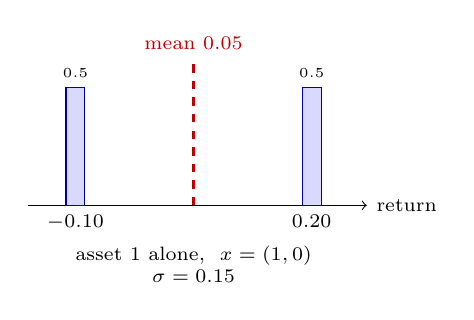
\begin{tikzpicture}[scale=1.0, font=\scriptsize]
  % x-coordinate = 10 x return, y-coordinate = 3 x probability
  \draw[->] (-1.6,0) -- (2.7,0) node[right] {return};
  \draw[fill=blue!15, draw=blue!65!black] (-1.12,0) rectangle (-0.88,1.5);
  \draw[fill=blue!15, draw=blue!65!black] (1.88,0) rectangle (2.12,1.5);
  \draw[dashed, red!75!black, thick] (0.5,0) -- (0.5,1.85) node[above] {mean $0.05$};
  \node[below] at (-1,0) {$-0.10$}; \node[below] at (2,0) {$0.20$};
  \node[above, font=\tiny] at (-1,1.5) {$0.5$}; \node[above, font=\tiny] at (2,1.5) {$0.5$};
  \node[align=center] at (0.5,-0.75) {asset 1 alone, \ $x = (1, 0)$\\ $\sigma = 0.15$};
\end{tikzpicture}
\hspace{16mm}
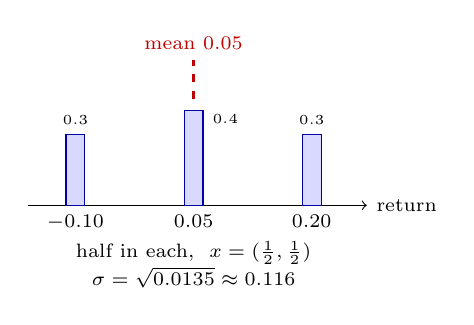
\begin{tikzpicture}[scale=1.0, font=\scriptsize]
  \draw[->] (-1.6,0) -- (2.7,0) node[right] {return};
  \draw[fill=blue!15, draw=blue!65!black] (-1.12,0) rectangle (-0.88,0.9);
  \draw[fill=blue!15, draw=blue!65!black] (0.38,0) rectangle (0.62,1.2);
  \draw[fill=blue!15, draw=blue!65!black] (1.88,0) rectangle (2.12,0.9);
  \draw[dashed, red!75!black, thick] (0.5,1.35) -- (0.5,1.85) node[above] {mean $0.05$};
  \node[below] at (-1,0) {$-0.10$}; \node[below] at (0.5,0) {$0.05$}; \node[below] at (2,0) {$0.20$};
  \node[above, font=\tiny] at (-1,0.9) {$0.3$}; \node[right, font=\tiny] at (0.62,1.1) {$0.4$};
  \node[above, font=\tiny] at (2,0.9) {$0.3$};
  \node[align=center] at (0.5,-0.75) {half in each, \ $x = (\tfrac12, \tfrac12)$\\ $\sigma = \sqrt{0.0135} \approx 0.116$};
\end{tikzpicture}
\end{center}
\vspace{4pt}

\quad same mean, less spread: \textbf{diversification}. \ it comes from $\rho < 1$ --- with $\rho = 1$, \ $x^{\top}\Sigma x$ would stay $0.0225$.
\vspace{12pt}

\textbf{The model} \quad (Markowitz, 1952) \quad --- least risk, subject to an expected-return target $r$:
\[
\begin{aligned}
  \min_x\quad & x^{\top}\Sigma x && \text{variance of the return (risk)}\\
  \text{s.t.}\quad & \mu^{\top}x \ge r && \text{expected return meets the target}\\
                   & \mathbf{1}^{\top}x = 1, \quad x \ge 0 && x \in X
\end{aligned}
\]

\quad Section 5's QP with $Q = 2\Sigma$, $c = 0$; \ convex because $\Sigma \succeq 0$ (Section 6).
\vspace{3pt}

\quad in the language of the bridge: the loss $-\tilde\xi^{\top}x$ is random; Markowitz collapses it with two numbers ---
\vspace{1pt}

\qquad its variance (objective) and its mean (constraint).
\vspace{12pt}

\textbf{Data --- the coding session} \quad $n = 3$, \ $r = 0.10$
\vspace{5pt}

\begin{center}
\begin{tabular}{@{}l|c|c|c@{}}
 asset $j$ & expected return $\mu_j$ & variance $\Sigma_{jj}$ & $\sigma_j = \sqrt{\Sigma_{jj}}$ \\ \hline
 bond      & $0.06$ & $0.010$ & $0.10$ \\
 tech      & $0.10$ & $0.040$ & $0.20$ \\
 energy    & $0.15$ & $0.090$ & $0.30$ \\
\end{tabular}
\end{center}
\vspace{4pt}

\[
x = \begin{pmatrix} x_{\text{bond}} \\ x_{\text{tech}} \\ x_{\text{energy}} \end{pmatrix},
\qquad
\mu = \begin{pmatrix} 0.06 \\ 0.10 \\ 0.15 \end{pmatrix},
\qquad
\Sigma = \begin{pmatrix} 0.010 & 0.001 & 0 \\ 0.001 & 0.040 & 0.015 \\ 0 & 0.015 & 0.090 \end{pmatrix}
\]

\quad covariances: \ bond--tech $0.001$, \ tech--energy $0.015$, \ bond--energy $0$
\vspace{6pt}

\quad written out term by term --- exactly the lines typed in the code:
\[
\begin{aligned}
  \min\quad & 0.010\,x_{\text{bond}}^2 + 0.040\,x_{\text{tech}}^2 + 0.090\,x_{\text{energy}}^2
              + 2(0.001)\,x_{\text{bond}}x_{\text{tech}} + 2(0.015)\,x_{\text{tech}}x_{\text{energy}} \\
  \text{s.t.}\quad & 0.06\,x_{\text{bond}} + 0.10\,x_{\text{tech}} + 0.15\,x_{\text{energy}} \ge 0.10 \\
                   & x_{\text{bond}} + x_{\text{tech}} + x_{\text{energy}} \le 1 \\
                   & x_{\text{bond}},\ x_{\text{tech}},\ x_{\text{energy}} \ge 0
\end{aligned}
\]

\quad budget ``$\le 1$'': leftover sits in cash earning $0$ --- never helps, so the sum is $1$ at the optimum
\vspace{6pt}

\textbf{Solution}
\vspace{3pt}

\quad $\boxed{x^{\star} \approx (0.39,\ 0.29,\ 0.31), \qquad x^{\star\top}\Sigma x^{\star} \approx 0.0169, \qquad \sigma \approx 0.130}$
\qquad $\mu^{\top}x^{\star} = 0.10$ --- target met exactly
\vspace{4pt}

\quad all in tech: \ same expected return $0.10$, \ but $\sigma = 0.20$. \quad the mix cuts $\sigma$ by about a third.
\vspace{3pt}

\quad every asset gets a share --- not a vertex (Section 5).
\vspace{6pt}

\begin{center}
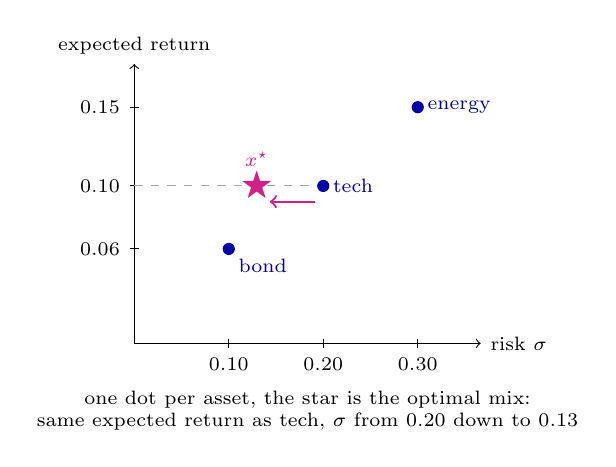
\begin{tikzpicture}[scale=1.0, font=\scriptsize]
  % x-coordinate = 12 x sigma, y-coordinate = 20 x mean
  \draw[->] (0,0) -- (4.4,0) node[right] {risk $\sigma$};
  \draw[->] (0,0) -- (0,3.55) node[above] {expected return};
  \foreach \s/\lab in {1.2/0.10, 2.4/0.20, 3.6/0.30}
    { \draw (\s,0.06) -- (\s,-0.06) node[below] {$\lab$}; }
  \foreach \m/\lab in {1.2/0.06, 2.0/0.10, 3.0/0.15}
    { \draw (0.06,\m) -- (-0.06,\m) node[left] {$\lab$}; }
  \draw[dashed, gray!70] (0,2.0) -- (2.4,2.0);
  \fill[blue!65!black] (1.2,1.2) circle (2.2pt) node[below right] {bond};
  \fill[blue!65!black] (2.4,2.0) circle (2.2pt) node[right] {tech};
  \fill[blue!65!black] (3.6,3.0) circle (2.2pt) node[right] {energy};
  \draw[->, magenta!85!black, thick] (2.3,1.8) -- (1.72,1.8);
  \node[magenta!85!black] at (1.558,2.0) {\large$\bigstar$};
  \node[anchor=south, magenta!85!black] at (1.558,2.12) {$x^{\star}$};
  \node[align=center] at (2.2,-0.85) {one dot per asset, the star is the optimal mix:\\ same expected return as tech, $\sigma$ from $0.20$ down to $0.13$};
\end{tikzpicture}
\end{center}
\end{board}
\end{board}
\demo{week03\_markowitz.ipynb}{Colab --- build this model live from the skeleton, then compare with the completed cell.}
\demo{demos/markowitz\_portfolio.py}{the same model as a plain script: prints the model, solves it, plots the weights $x^{\star}$.}
\takeaway{the running example: the loss $-\tilde\xi^{\top}x$ stays; each later model changes only how it is collapsed to a number --- today variance, next CVaR and VaR.}

%% ---------------------------------------------------------------- next
\par\medskip
{\color{ruleink}\rule{\textwidth}{1.2pt}}\par\nobreak\vspace{3pt}
{\color{keyink}\small\textbf{next}\quad no class Sep 26. \ week 6 --- duality: every LP comes with a shadow LP, and why $\max = \min$.}

\end{document}
